\documentclass[12pt]{article}

\usepackage{amsmath}
\usepackage{graphicx}
\usepackage{hyperref}
\usepackage[margin=1.2in]{geometry}

\providecommand{\eqn}[1]{eqn.~(\ref{eqn:#1})}
\providecommand{\tab}[1]{Table~\ref{tab:#1}}
\providecommand{\fig}[1]{Figure~\ref{fig:#1}}

\providecommand{\vecsymbol}[1]{\ensuremath{\boldsymbol{#1}}}
\providecommand{\pv}{\vecsymbol{p}}
\providecommand{\deltav}{\vecsymbol{\delta}}

\title{Co-Addition of Spectro-perfect\\
Reductions for DESI\\
\vspace{5mm}{\large\bf DESI-doc-????}}
\author{David Kirkby}

\begin{document}
\maketitle

\section{Introduction}

In this note, ~\cite{2010PASP..122..248B}. We start with an overview of the data flow from individual DESI exposures to final co-added spectra. We next review the spectroperfectionism algorithm and our assumptions about the inputs to be co-added. Finally, we describe the two phases of our co-addition algorithm: combining the exposures from a single camera (b,r,z) and then combining per-camera co-adds to obtain the final spectrum.

This document is maintained in the {\tt desispec} package\footnote{Maintained in the public github repository at \url{https://github.com/desihub/desispec}} under {\tt doc/tex/} and the code for the plots and toy studies described below are maintained in an iPython notebook under {\tt doc/nb/}\footnote{Viewable online at \url{http://nbviewer.ipython.org/github/desihub/desispec/tree/master/doc/nb/SpectroPerfectCoadds}}.

\section{Dataflow Overview}

\fig{dataflow} summarizes the basic flow of spectra from the nightly observations to the global coadds. The primary temporal key is the dataflow is the exposure ID, a global integer counter that increments over the course of the survey. The primary spatial key is the object identifier, a 64-bit integer assigned during the targeting phase. For convenience, these are currently chunked into ``nights'' and ``bricks'', respectively, although the current design does not provide efficient means to determine either of these from the primary keys. An additional element of the data flow not shown explicitly in \fig{dataflow} is the targeting metadata contained within per-exposure fibermap files. The per-exposure meta data associated with each target follows an identical flow to its associated reduced spectrum (represented by estimates of the object's flux, inverse variance, and resolution).

\begin{figure}[htb]
\begin{center}
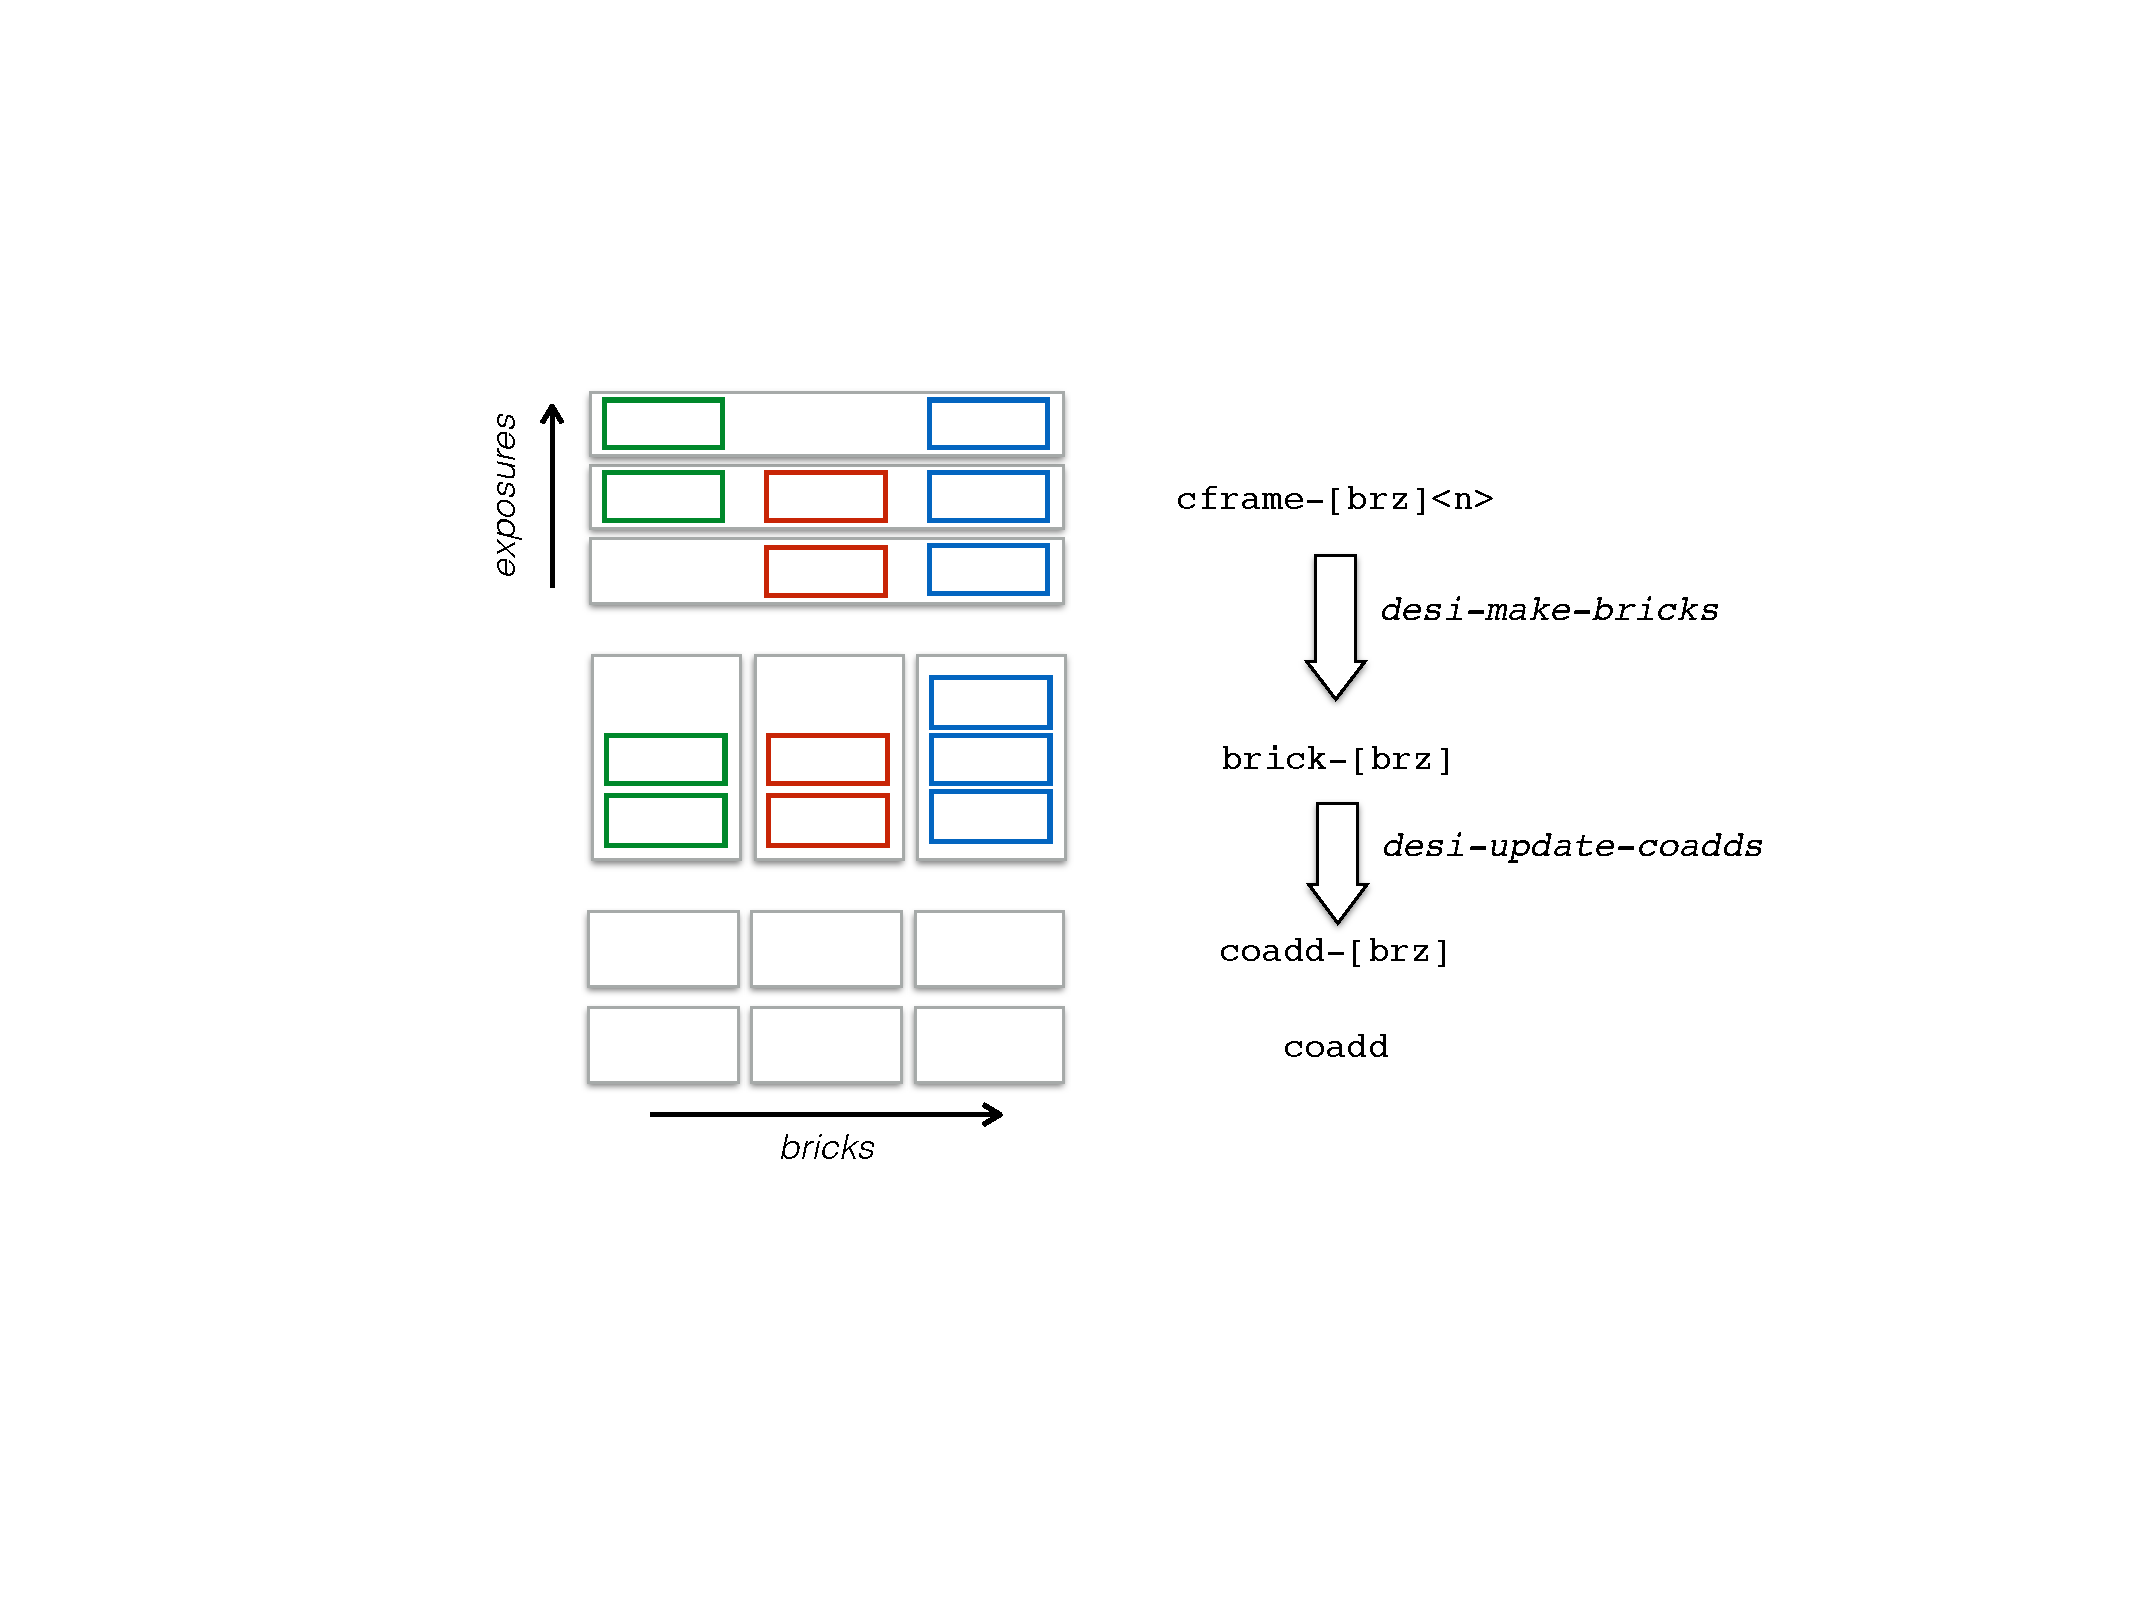
\includegraphics[width=5in]{fig/dataflow}
\caption{Schematic representation of the coaddition dataflow. Nightly exposures are reduced to cframes (horizontal gray boxes) each covering multiple bricks (colored boxes). The {\tt desi-make-bricks} program repackages the cframe spectra into brick files (vertical gray boxes) containing all of the spectra observed for targets within a single brick. Finally, the {\tt desi-update-coadds} program reads spectra from a single brick file and generates the per-band and global coadd files (gray boxes at the bottom of the diagram).}
\label{fig:dataflow}
\end{center}
\end{figure}

Note that there is a certain amount of duplication of information in this data flow, by design. For example, single-exposure spectra and their associated metadata are duplicated in cframe and brick files, but with different groupings. Also, the fibermap metadata is duplicated at each stage of the processing so that, for example, end users of global coadds can work with a single data product and do not need to retrace the processing steps to determine provenance.

\section{Spectro-Perfect Reductions}

The reduction algorithm assumes that the mean pixel values due to a true object flux are related by a linear transform
\begin{equation}
\langle \pv \rangle = A f + \deltav \; ,
\end{equation}
where $A$ is a rectangular matrix that incorporates the results of arc and flat calibrations to transform an incident flux vector $f$ into a (flattened) vector $\pv$ of pixel values\footnote{We use boldface to distinguish flattened vectors in pixel space from vectors in wavelength space.} and $\deltav$ represents the mean dark current. With pixel values given in units of detected electrons, the corresponding covariance is then diagonal
\begin{equation}
N \equiv \langle\pv \pv^T\rangle = \text{diag}\left( A f + \deltav + \sigma^2_{r} \right) \; ,
\end{equation}
where $\sigma_r$ is the RMS read noise in equivalent electron units, which is assumed to be uncorrelated between pixels. The maximum likelihood estimator for $f$ is then given by the solution of the least-squares problem
\begin{equation}
C^{-1} f = A^T N^{-1} \pv
\label{eqn:leastsq}
\end{equation}
with a flux inverse covariance given by
\begin{equation}
C^{-1} = A^T N^{-1} A \; .
\end{equation}
The least-square solution effectively deconvolves the instrumental PSF and inevitably leads to large oscillations on scales $\Delta\lambda$ smaller than the resolution that are unconstrained by $\pv$. One approach to this problem is to add a regularization term to \eqn{leastsq} that imposes a smoothness prior on $f$.  The spectro-perfectionism approach is instead to find a diagonal basis for the flux inverse covariance,
\begin{equation}
C^{-1} = R^T \tilde{C}^{-1} R \; ,
\label{eqn:decorrelated}
\end{equation}
in which the transformed flux components
\begin{equation}
\tilde{f} \equiv R f
\end{equation}
are uncorrelated, i.e., $\tilde{C}^{-1}$ is diagonal. Any real-valued square matrix (not necessarily orthogonal) that satisfies \eqn{decorrelated} is a valid decorrelation of $C^{-1}$. Furthermore, there are an infinite number of ways to accomplish this since, given one $R$, we can always find another solution
\begin{equation}
R^T \tilde{C}^{-1} R = S^T \tilde{D}^{-1} S \; ,
\end{equation}
where
\begin{equation}
S = \tilde{D}^{+1/2} O \tilde{C}^{-1/2} R
\end{equation}
for an arbitrary orthogonal matrix $O$ and positive diagonal matrix $\tilde{D}$. However, some natural choices for $R$ are the matrix of eigenvalues, the Cholesky decomposition, and the matrix square root. As explained in reference~\cite{2010PASP..122..248B} (and earlier demonstrated in reference~\cite{2000MNRAS.312..285H} in a different context), the matrix square root is a good choice since the resulting $R$ generally has the properties of a resolution matrix when suitably normalized: each component is $f$ is transformed to a narrow range of nearby wavelengths.

For the co-addition tests described below, we construct toy response matrices $A_i$ for a three-fiber spectrograph with rather extreme PSF variations along each trace, as illustrated in \fig{detector} below. Responses are simulated using the GalSim package~\cite{2014arXiv1407.7676R}. Note that each fiber $i$ has its response matrix that reflects the range of pixels it illuminates above some threshold, as illustrated by the upper plot of~\fig{detector}.  There is inevitably some cross talk between fibers that can either be handled by assigning overlap pixels to more than one $A_i$ and then propagating correlated uncertainties, or else by uniquely assigning each pixel to its most relevant fiber and then accepting some corresponding systematic error due to un-modeled leakage. Note that pixels with very small relative responses (shown in gray) must be eliminated from the response matrix to improve the numerical stability of the resulting least-squares problem.

\begin{figure}[htb]
\begin{center}
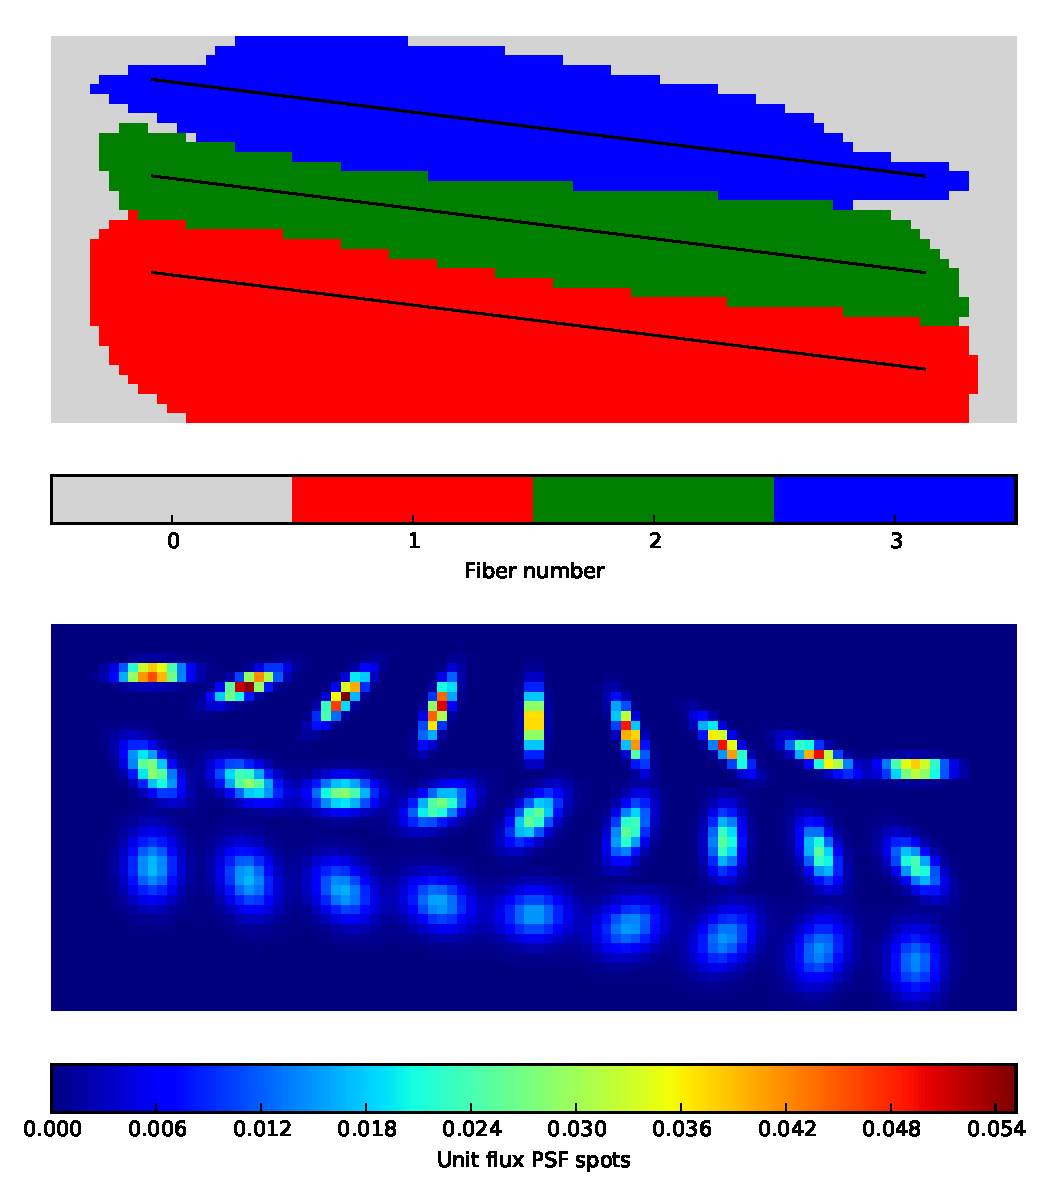
\includegraphics[width=5.5in]{fig/detector}
\caption{Simulated detector response for a three-fiber spectrograph. The upper plot shows the map between CCD pixels and fibers used to construct the three response matrices, with grey pixels not assigned to any fiber. The three fiber traces are superimposed as black lines. The lower plot shows representative PSF spots along each trace, exhibiting large variations in size and shape for the purposes of demonstration.}
\label{fig:detector}
\end{center}
\end{figure}

\section{Co-Addition}

The goal of co-addition is to optimally combine statistically independent observations of the same object, which naturally suggests an appropriately weighted mean. For a given object with true flux $f$, the pipeline provides reduced a reduced flux $\tilde{f}_{ij}$ for a set of exposures $i$ and cameras $j$, together with its associated resolution matrix $R_{ij}$ and diagonal inverse covariance matrix $\tilde{C}_{ij}$. Each reduced flux $\tilde{f}_{ij}$ is an estimator of the resolution-convolved true object flux $R_{ij} f$, so the appropriate weighted average here is of deconvolved reduced fluxes $R_{ij}^{-1} \tilde{f}_{ij}$. Specifically, we first accumulate the weighted sums for each camera
\begin{align}
C_j^{-1} &= \sum_i C_{ij}^{-1} = \sum_i R_{ij}^T \tilde{C}_{ij}^{-1} R_{ij} \\
C_j^{-1}f &= \sum_i C_{ij}^{-1} f = \sum_i R_{ij}^T \tilde{C}_{ij}^{-1} \tilde{f}_{ij} \; .
\end{align}
Next, we find the unique decorrelated decomposition of $C_j^{-1} = R_j^t \tilde{C}_j R_j$, using the same method described above, and then calculate the corresponding decorrelated flux $\tilde{f}_j$ in each camera as
\begin{equation}
\tilde{f}_j = R_j f = \tilde{C_j} (R_j^T)^{-1} \left( C_j^{-1}f \right)
= \tilde{C_j} (R_j^T)^{-1} \sum_i R_{ij}^T \tilde{C}_{ij}^{-1} \tilde{f}_{ij}\; .
\end{equation}

Note that the final right-hand expressions in the equations above are all calculated directly in terms of the per-exposure pipeline outputs ($R_{ij}$, $\tilde{C}_{ij}^{-1}$, $\tilde{f}_{ij}$), so there is never any need to evaluate the numerically unstable deconvolution $R_{ij}^{-1} \tilde{f}_{ij}$. There are two steps to this algorithm with potential numerical issues: the decorrelated decomposition of $C_j^{-1}$ and the subsequent inversion of $R_j^T$. However, both of these steps should present no problems when the individual $R_{ij}$ and $\tilde{C}_{ij}$ inputs are valid (i.e., the corresponding $C_{ij}^{-1}$ is positive definite and well conditioned), and can even succeed for some types of invalid input due to the summations (for example, a few exposures with some zero inverse variances).

\fig{repeats} shows the results of co-adding four exposures of the detector shown in~\fig{detector}, where the detector configuration ($A$ and $\deltav$) is held constant and only the noise varies between exposures. Note that the different resolutions for each fiber are evident in the smoothing of the narrow peak, and that the co-add has the same resolution as the individual exposures (since this is determined by the intrinsic detector responses rather than by the signal to noise ratio). Also note that the co-add errors are roughly half the width of the single-exposure error band, as expected.

\begin{figure}[htb]
\begin{center}
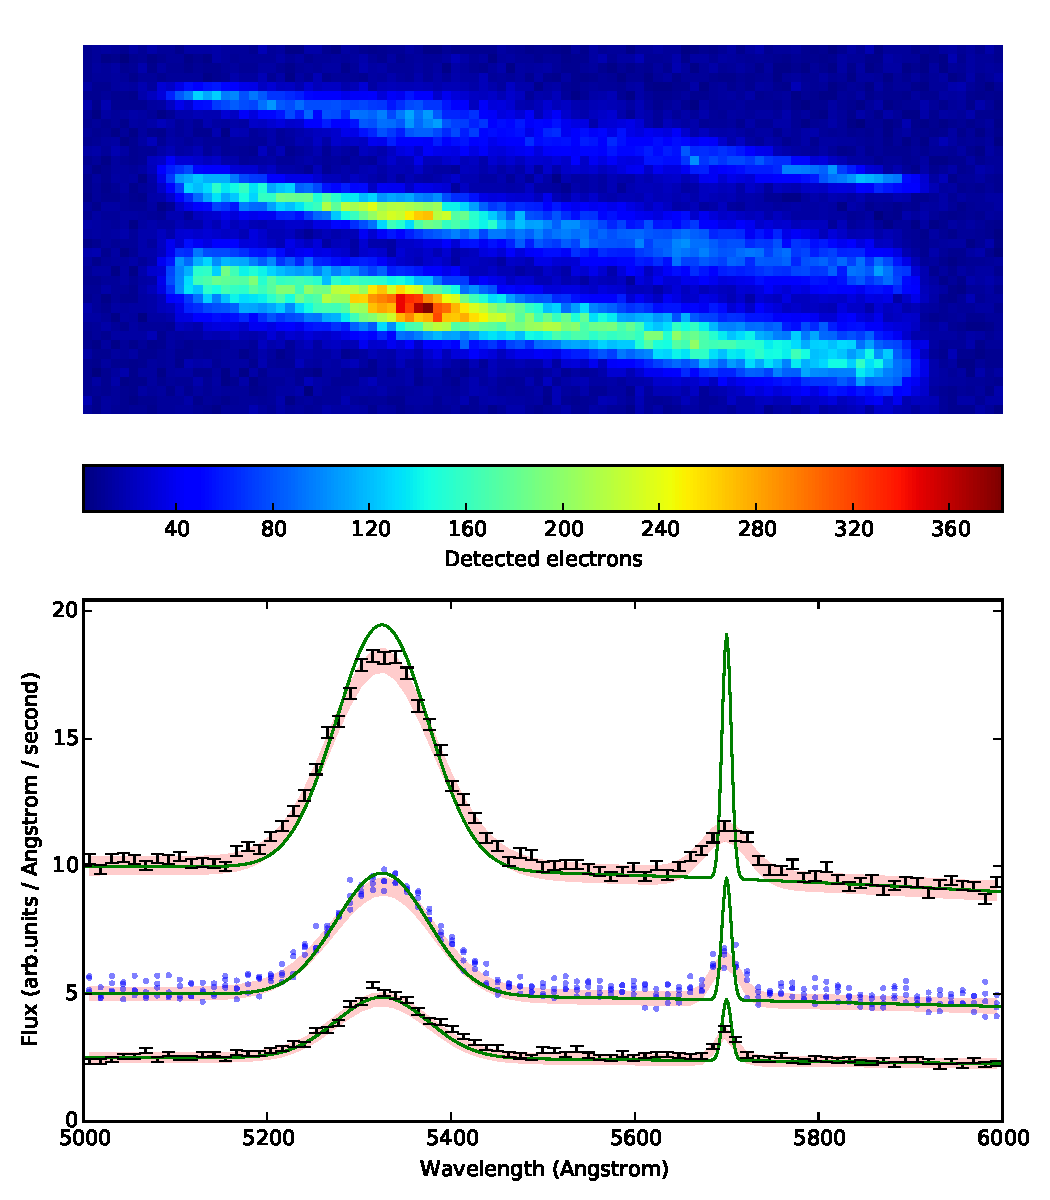
\includegraphics[width=5.5in]{fig/repeats}
\caption{Co-addition of four simulated repeat exposures. The upper plot shows one simulated exposure and the lower plot shows the four reductions for each fiber. The simulation uses the same source SED shape for each fiber but with different normalizations, as shown with the green curves.  The shaded red bands show the resolution-convolved true fluxes $R_1 f$ for the first exposure ($i=1$), with a width corresponding to the diagonal errors $\tilde{C_1}^{1/2}$. Error bars on the top and bottom spectra show the four-exposure co-adds, while blue points show the scatter of the single-exposure reductions.}
\label{fig:repeats}
\end{center}
\end{figure}

We next test co-adds where the detector configuration and integration time vary between exposures... Note that by requiring that co-added fluxes be decorrelated, we are generally degrading the resolution of the best individual observations...

\begin{figure}[htb]
\begin{center}
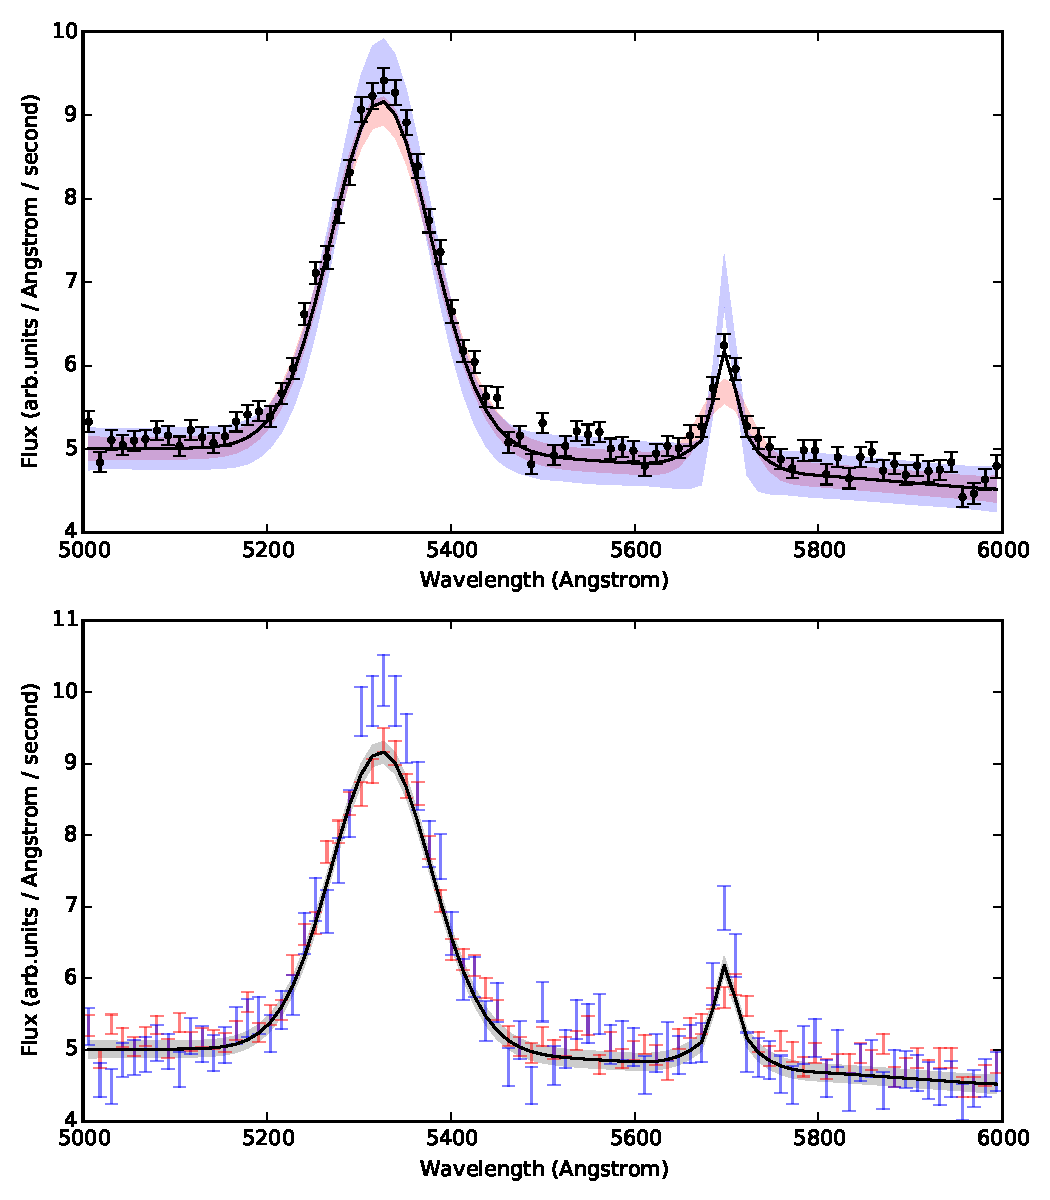
\includegraphics[width=5.5in]{fig/stacked}
\caption{Co-addition of two simulated exposures with different detector configurations and integration times. The upper plot shows the calculated error bands for each exposure, centered on the true resolution-convolved flux, with the true-resolution convolved co-added flux shown as a solid black curve and the decorrelated coadded fluxes superimposed with their diagonal inverse-covariance errors. The lower plot shows the calculated error band for the coadd, centered on the true resolution-convolved flux, with the individual exposure decorrelated fluxes superimposed with their diagonal inverse-covariance errors.}
\label{fig:stacked}
\end{center}
\end{figure}

Our final step is to combine the co-adds for each camera, which introduces two new ingredients to the algorithm described above: first, some wavelengths ranges will be missing from each exposure and, second, where wavelength coverages overlap, the reduced flux will generally be sampled on different grids. We ultimately want a combined flux sampled on a single global grid covering the full wavelength range of the cameras. We therefore define a resampling matrix $S_j$ that converts a vector sampled on the global wavelength grid to one sampled on the local grid of camera $j$ via the linear transform
\begin{equation}
f_j = S_j f \; .
\end{equation}
For concreteness, we use an $S_j$ that implements linear interpolation but higher-order interpolation schemes can also be accommodated in the same framework. The inverse covariance of deconvolved flux estimates on the global grid due to camera $j$ is then
\begin{equation}
S_j^T C_j^{-1} S_j = S_j^T R_j^T \tilde{C}_j^{-1} R_j S_j \; ,
\end{equation}
which assigns zero inverse covariance (i.e., no information) to wavelengths outside the camera's coverage. We now proceed just as above: first, accumulate the weighted sums
\begin{align}
C^{-1} &= \sum_j S_j^T R_j^T \tilde{C}_j^{-1} R_j S_j \label{eqn:step2cinv} \\
C^{-1}f &= \sum_j S_j^T R_j^T \tilde{C}_j^{-1} \tilde{f}_j \; ,
\end{align}
then decorrelate
\begin{equation}
C^{-1} = R^T \tilde{C} R \; ,
\end{equation}
and finally calculate the co-added decorrelated flux
\begin{equation}
\tilde{f} = \tilde{C} (R^T)^{-1} \sum_j S_j^T R_j^T \tilde{C}_j^{-1} \tilde{f}_j \; .
\label{eqn:step2}
\end{equation}
This second step of co-addition places some constraints on the choice of global wavelength grid in order that \eqn{step2cinv} be positive definite: roughly speaking, we require that the gobal grid be no more dense than the combined individual camera grids and not extend beyond camera's coverage. In practice, we require an algorithm that can handle masked pixels or even a missing camera, which will generally yield an invalid $C^{-1}$. We allow for these defects by pruning any rows of $C^{-1}$ that are identically zero before the decorrelation step, and then re-inserting these rows with zero entries in $\tilde{C}$ and $R$.

\fig{global} shows a test of this algorithm for three simulated cameras with overlapping wavelength coverages. In this example, all three cameras use uniformly spaced wavelength grids with different spacings.  The global wavelength grid matches the spacing of the blue camera's grid so we can check that the coadd is an identity transform for $\lambda < 5200$ \AA\ where only the blue camera contributes. As a test, we have masked out two regions of the red camera's coverage. This results in larger co-added errors in the region near 5300 \AA\, as expected. More surprisingly, the coadd provides flux estimates with non-zero inverse covariance in the region near 5550 \AA\, even though there are no overlapping pixels from a second camera: this is due to width of the resolution function which allows nearby wavelengths to constrain the missing fluxes, although with smaller weights and correspondingly larger errors.

\begin{figure}[htb]
\begin{center}
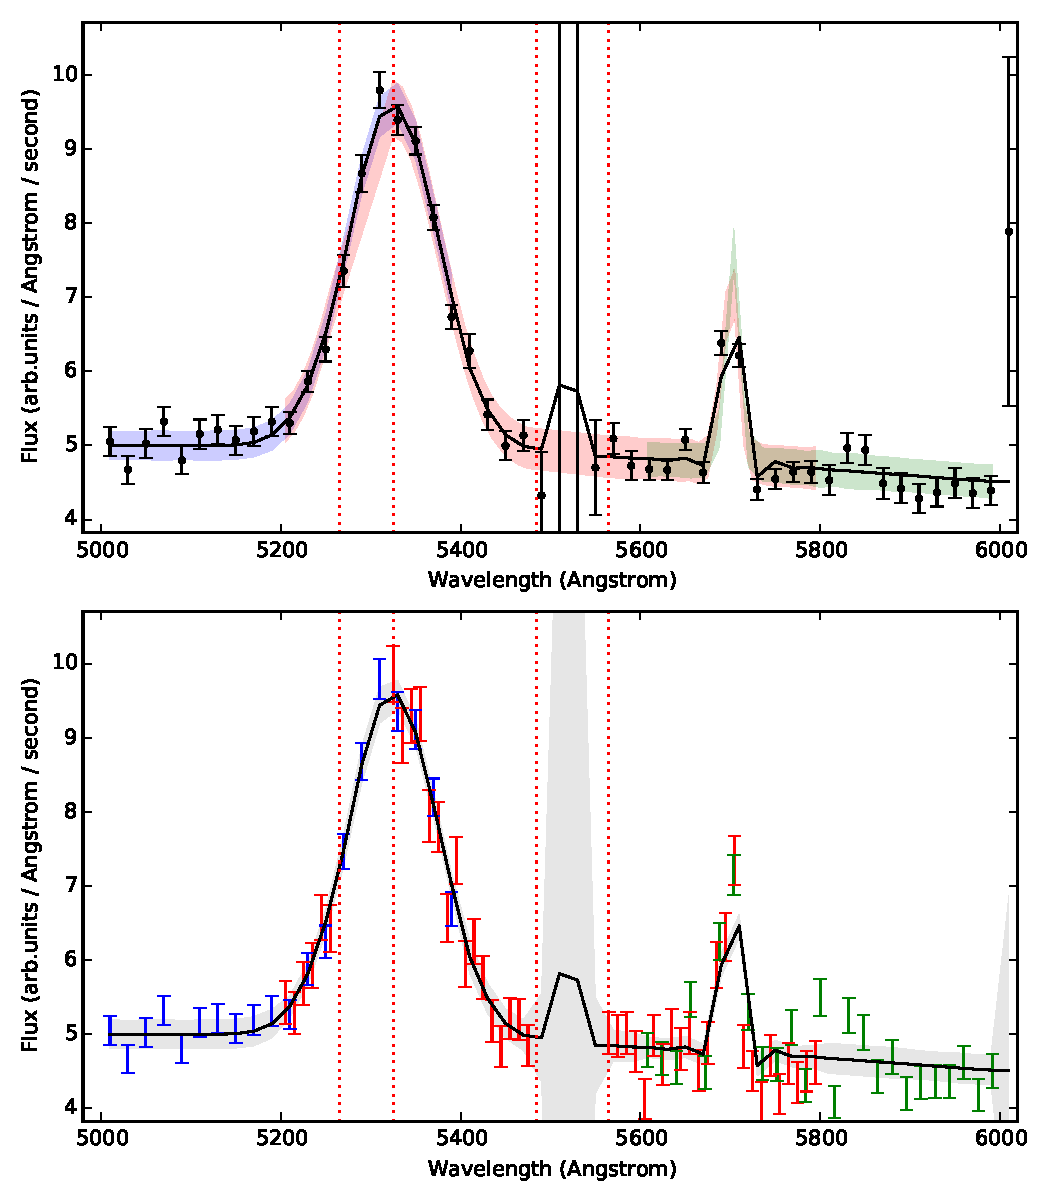
\includegraphics[width=5.5in]{fig/global}
\caption{Co-addition of reductions for three overlapping cameras, indicated using blue, red, and green. This plot uses the same format as~\fig{stacked} except that there are now three spectra being coadded, and the individual exposures and the coadd all have different wavelength grids. Vertical dotted red lines show regions where red-camera pixels have been masked out to demonstrate how this impacts the coadded result.}
\label{fig:global}
\end{center}
\end{figure}

We adopt a uniformly spaced wavelength grid for the final DESI coadds with 1.0 \AA\ per bin. This is a compromise between spectrum size (otherwise, we could go down to the 0.6 \AA\ spacing of the idividual bands) and a desire to maintain a roughly constant ratio between the wavelength PSF size and the bin size. \fig{grids} shows that an alternative global grid that is equally spaced in in $\log\lambda$ is not a good match to the PSF size, especially at the red ends of the r-band and z-band. This means that a redshift estimator that requires $\log\lambda$ spacing will need to resample as a preprocessing step.

\begin{figure}[htb]
\begin{center}
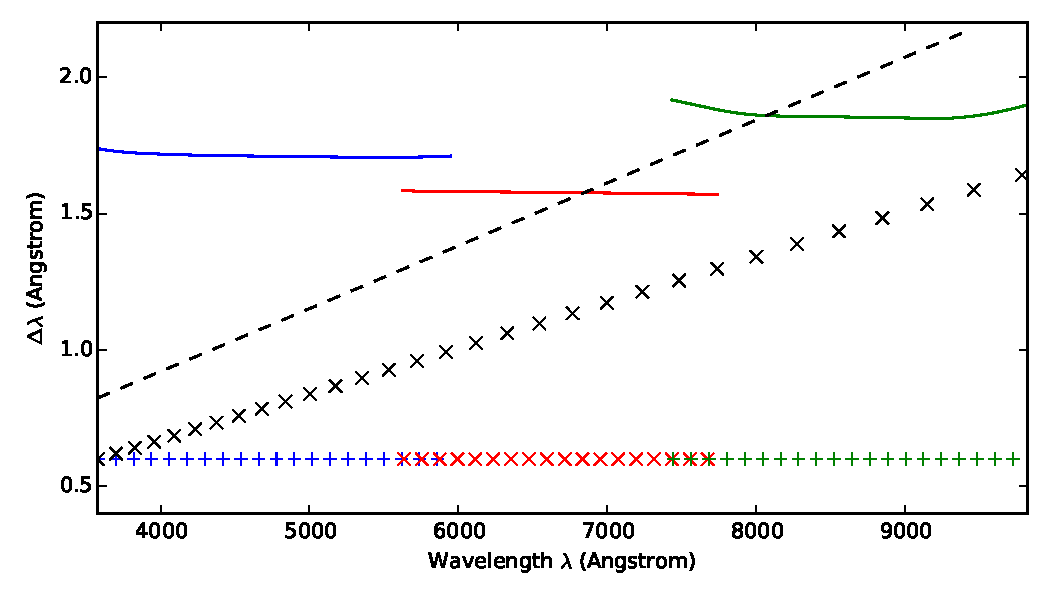
\includegraphics[width=5in]{fig/grids}
\caption{Comparison of different wavelength grids. The horizontal row at $\Delta\lambda = 0.6$ \AA\ shows the local grids used in the DESI b,r,z cameras (with one point per 200 bins) while the solid curves show the corresponding wavelength PSF FWHM values. The two rising lines show global grids that are equally spaced in $\log\lambda$: crosses show a possible global binning for DESI that starts at $\Delta\lambda = 0.6$ \AA\ and the dashed line shows the coadd grid used by BOSS. The horizontal row at $\Delta\lambda = 1.0$ \AA\ shows the global DESI coadd grid.}
\label{fig:grids}
\end{center}
\end{figure}

As a final note, we remind readers that the decomposition of a spectro-perfect reduction into separate flux, inverse variance, and resolution components is somewhat arbitrary since these quantities are highly correlated. In principle, the matrix square-root prescription provides a unique decomposition. However, in practice the presence of round off errors in operations on matrices with $~4000^2$ elements (or $~6000^2$ for the global coadd) leads to percent-level uncertainties in the decomposition results.  This is illustrated in~\fig{roundtrip}, where we plot the shifts in flux, inverse variance, and resolution values under a single decorrelation round trip via
\begin{equation}
R^T \tilde{C}^{-1} R \rightarrow C^{-1} \rightarrow R^T \tilde{C}^{-1} R
\end{equation}
and
\begin{equation}
f \rightarrow \tilde{C} (R^T)^{-1} \left( R^T \tilde{C}^{-1} f \right) \rightarrow f \; .
\end{equation}

\begin{figure}[htb]
\begin{center}
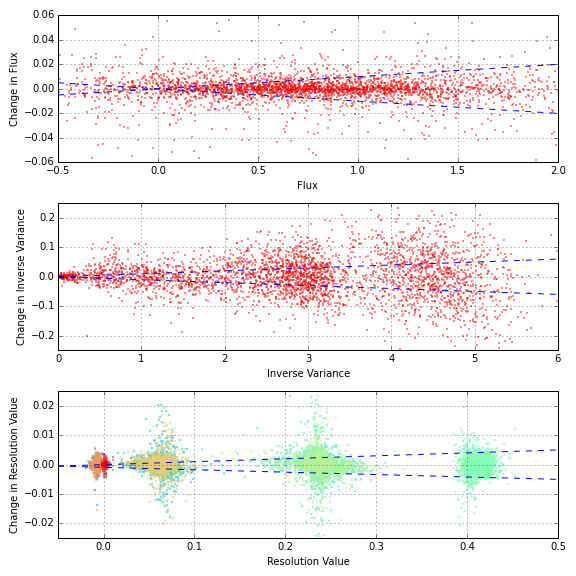
\includegraphics[width=5in]{fig/roundtrip}
\caption{Shifts in flux (top), inverse variance (middle) and resolution matrix values (bottom) from a decorrelation round trip. Dashed blue lines represent fractional shifts of $\pm 1$\%. The different colored clusters in the bottom plot are for resolution matrix elements on different off-diagonals.}
\label{fig:roundtrip}
\end{center}
\end{figure}

\def\apjl{ApJL} %Astrophysical Journal Letters
\def\aj{AJ} %Astronomical Journal
\def\apj{ApJ} %Astrophysical Journal
\def\pasp{PASP} %Publications of the Astronomical Society of the Pacific
\def\spie{SPIE} %
\def\apjs{ApJS} %Astrophysical Journal Supplement
\def\araa{ARAA} %Annual Review of Astronomy and Astrophysics
\def\aap{A\&A} %Astronomy and Astrophysics
\def\aaps{A\&A~Supl.} %Astronomy and Astrophysics Supplement
\def\nat{Nature} %Nature
\def\nar{New Astron. Rev.} %New Astronomy Review
\def\mnras{MNRAS} %Monthly Notices of the Royal Astronomical Society
\def\jcap{JCAP} %Journal of Cosmology and Astroparticle physics
\def\prd{{Phys.~Rev.~D}}        % Physical Review D
\def\physrep{{Phys.~Reports}} % Physics Reports

\bibliographystyle{plain}
\bibliography{coadd}

\end{document}
